\documentclass[8pt,a4paper,compress,handout]{beamer}

\usepackage{/home/siyer/lib/slides}

\title{Recursion}
\date{}

\begin{document}
\begin{frame}
\begin{flushright}
\tiny \textsc{To iterate is human, to recurse divine. \\ - L. Peter Deutsch}
\end{flushright}
\titlepage
\end{frame}

\begin{frame}
\frametitle{Outline}
\tableofcontents
\end{frame}

\section{.}
\begin{frame}[fragile]
\begin{framed}
\tiny euclid.py: Accept integers $p$ and $q$ as command-line arguments, compute the greatest common divisor of $p$ and $q$, and write the result to standard output.
\end{framed}

\begin{lstlisting}[language=Python]
import stdio
import sys

def gcd(p, q):
    if q == 0:
        return p
    return gcd(q, p % q)

def main():
    p = int(sys.argv[1])
    q = int(sys.argv[2])
    divisor = gcd(p, q)
    stdio.writeln(divisor)

if __name__ == '__main__':
    main()
\end{lstlisting}

\begin{lstlisting}[language={}]
$ python euclid.py 1440 408
24
$ python euclid.py 314159 271828
1
\end{lstlisting}
\end{frame}

\begin{frame}[fragile]
\begin{framed}
\tiny towersofhanoi.py: Accept integer $n$ as a command-line argument. Write to standard output instructions to move $n$ Towers of Hanoi disks to the left.
\end{framed}

\begin{lstlisting}[language=Python]
import stdio
import sys

def moves(n, left):
    if n == 0:
        return
    moves(n - 1, not left)
    if left:
        stdio.writeln(str(n) + ' left')
    else:
        stdio.writeln(str(n) + ' right')
    moves(n - 1, not left)

def main():
    n = int(sys.argv[1])
    moves(n, True)

if __name__ == '__main__':
    main()
\end{lstlisting}

\begin{lstlisting}[language={}]
$ python towersofhanoi.py 3
1 left
2 right
1 left
3 left
1 left
2 right
1 left
\end{lstlisting}
\end{frame}

\begin{frame}[fragile]
\begin{framed}
\tiny beckett.py: Accept integer $n$ as a command-line argument. Write to standard output Beckett's stage instructions (the bit positions that change in a binary-reflected Gray code) for $n$ actors.
\end{framed}

\begin{lstlisting}[language=Python]
import stdio
import sys

def moves(n, enter):
    if n == 0:
        return
    moves(n - 1, True)
    if enter:
        stdio.writeln('enter ' + str(n))
    else:
        stdio.writeln('exit  ' + str(n))
    moves(n - 1, False)

def main():
    n = int(sys.argv[1])
    moves(n, True)

if __name__ == '__main__':
    main()
\end{lstlisting}

\begin{lstlisting}[language={}]
$ python beckett.py 3
enter 1
enter 2
exit  1
enter 3
enter 1
exit  2
exit  1
\end{lstlisting}
\end{frame}

\begin{frame}[fragile]
\begin{framed}
\tiny htree.py: Accept integer $n$ as a command-line argument. Draw a level $n$ H-tree centered at $(.5, .5)$ with lines of length $.5$.
\end{framed}

\begin{lstlisting}[language=Python]
import stddraw
import sys

def draw(n, lineLength, x, y):
    if n == 0:
        return
    x0 = x - lineLength / 2
    x1 = x + lineLength / 2
    y0 = y - lineLength / 2
    y1 = y + lineLength / 2
    stddraw.line(x0, y, x1, y)
    stddraw.line(x0, y0, x0, y1)
    stddraw.line(x1, y0, x1, y1)
    draw(n - 1, lineLength / 2, x0, y0)
    draw(n - 1, lineLength / 2, x0, y1)
    draw(n - 1, lineLength / 2, x1, y0)
    draw(n - 1, lineLength / 2, x1, y1)

def main():
    n = int(sys.argv[1])
    stddraw.setPenRadius(0.0)
    draw(n, .5, .5, .5)
    stddraw.show()

if __name__ == '__main__':
    main()
\end{lstlisting}
\end{frame}

\begin{frame}[fragile]
\begin{minipage}{160pt}
\begin{lstlisting}[language={}]
$ python htree.py 1
\end{lstlisting}
\end{minipage}%
\begin{minipage}{140pt}
\hfill 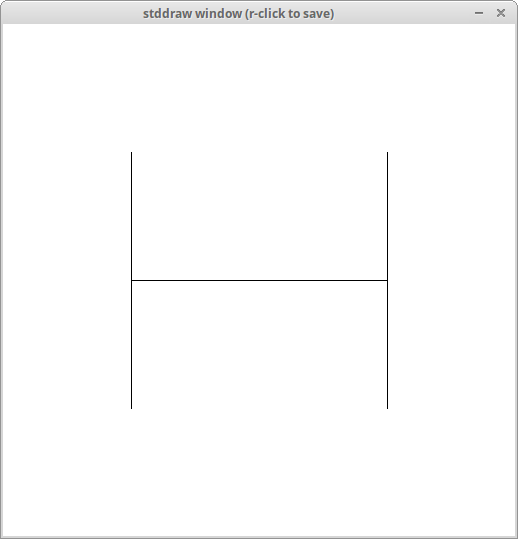
\includegraphics[scale=0.15]{figures/htree1.png}
\end{minipage}

\smallskip

\begin{minipage}{160pt}
\begin{lstlisting}[language={}]
$ python htree.py 3
\end{lstlisting}
\end{minipage}%
\begin{minipage}{140pt}
\hfill 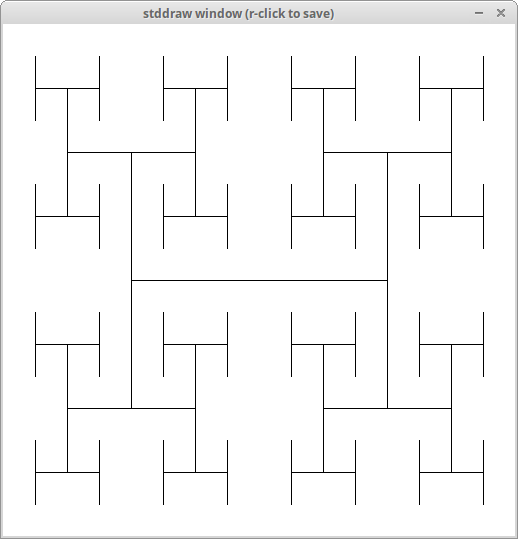
\includegraphics[scale=0.15]{figures/htree2.png}
\end{minipage}

\smallskip

\begin{minipage}{160pt}
\begin{lstlisting}[language={}]
$ python htree.py 5
\end{lstlisting}
\end{minipage}%
\begin{minipage}{140pt}
\hfill 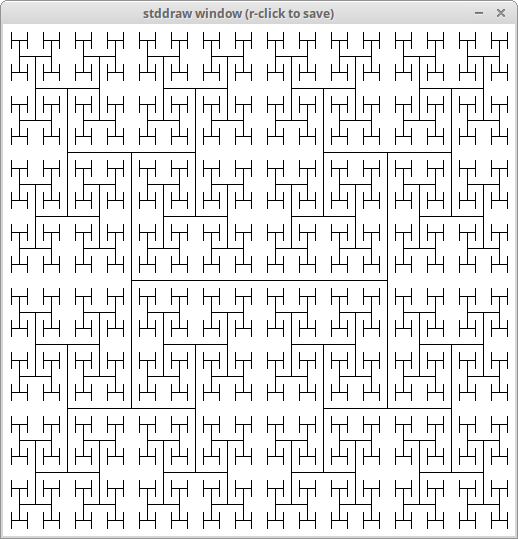
\includegraphics[scale=0.15]{figures/htree3.png}
\end{minipage}
\end{frame}

\begin{frame}[fragile]
\begin{framed}
\tiny brownian.py: Accept a Hurst exponent as a command-line argument. Use the Hurst exponent to compute a scale factor. Draw a Brownian bridge from $(0, .5)$ to $(1.0, .5)$ with variance $.01$ and that scale factor.
\end{framed}

\begin{lstlisting}[language=Python]
import math
import stddraw
import stdrandom
import sys

def curve(x0, y0, x1, y1, variance, scaleFactor):
    if (x1 - x0) < .01:
        stddraw.line(x0, y0, x1, y1)
        return
    xm = (x0 + x1) / 2.0
    ym = (y0 + y1) / 2.0
    delta = stdrandom.gaussian(0, math.sqrt(variance))
    curve(x0, y0, xm, ym + delta, variance / scaleFactor, scaleFactor)
    curve(xm, ym + delta, x1, y1, variance / scaleFactor, scaleFactor)

def main():
    hurstExponent = float(sys.argv[1])
    stddraw.setPenRadius(0.0)
    stddraw.clear(stddraw.LIGHT_GRAY)
    scaleFactor = 2 ** (2.0 * hurstExponent)
    curve(0, .5, 1.0, .5, .01, scaleFactor)
    stddraw.show()

if __name__ == '__main__':
    main()
\end{lstlisting}
\end{frame}

\begin{frame}[fragile]
\begin{minipage}{160pt}
\begin{lstlisting}[language={}]
$ python brownian.py 1
\end{lstlisting}
\end{minipage}%
\begin{minipage}{140pt}
\hfill 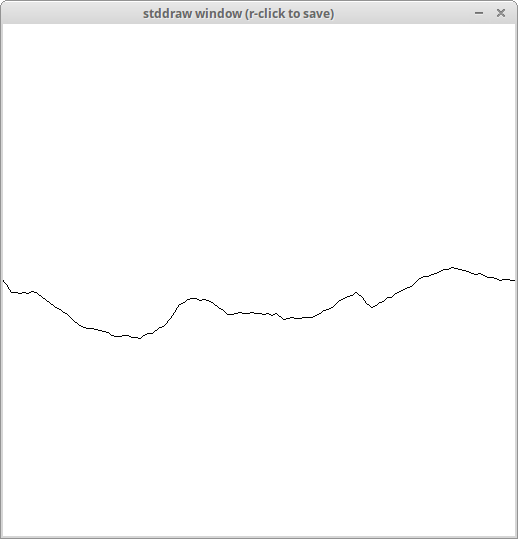
\includegraphics[scale=0.15]{figures/brownian1.png}
\end{minipage}

\smallskip

\begin{minipage}{160pt}
\begin{lstlisting}[language={}]
$ python brownian.py .5
\end{lstlisting}
\end{minipage}%
\begin{minipage}{140pt}
\hfill 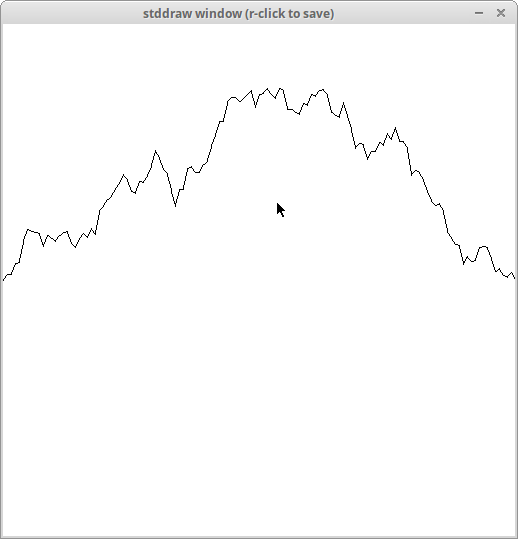
\includegraphics[scale=0.15]{figures/brownian2.png}
\end{minipage}

\smallskip

\begin{minipage}{160pt}
\begin{lstlisting}[language={}]
$ python brownian.py .05
\end{lstlisting}
\end{minipage}%
\begin{minipage}{140pt}
\hfill 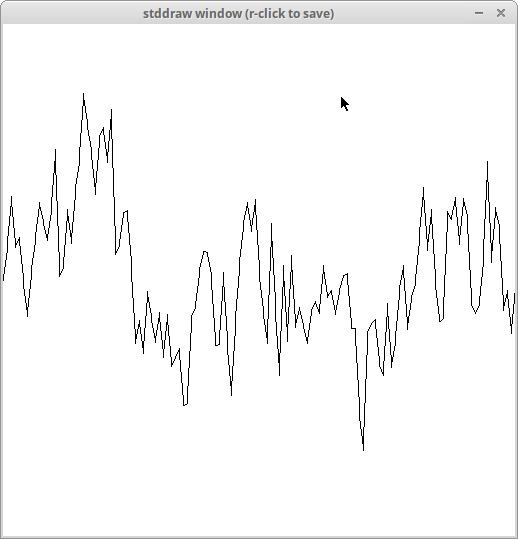
\includegraphics[scale=0.15]{figures/brownian3.png}
\end{minipage}
\end{frame}

\end{document}
